\documentclass{standalone}
\usepackage{tikz}
\usetikzlibrary{arrows,shapes,shadows,positioning}

\tikzset{
  %Define standard arrow tip
    >=stealth',
  %define style for boxes
  punkt/.style={
    rectangle,
    rounded corners,
    draw=black,very thick,
    text width=7.5em,
    minimum height = 2em,
    text centered},
  punkp/.style={
    rectangle,
    dashed,
    rounded corners,
    draw=black,very thick,
    text width=7.5em,
    text centered, 
    anchor=north,
    minimum height = 2em},
  %define style for arrows
  myarrow/.style={
    ->, 
    >=open triangle 90, 
    shorten >=1pt, 
    thick}
}


\begin{document}

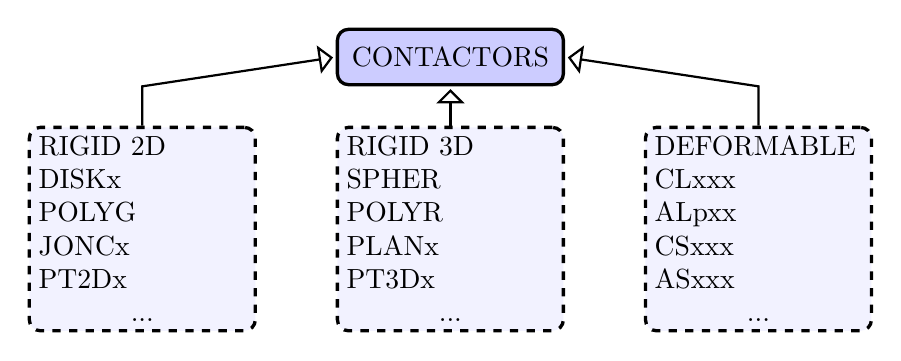
\begin{tikzpicture}[node distance=1cm, auto,]
%nodes
\node[punkt, fill=blue!20] (contactors) {CONTACTORS};

\node[punkp, below = 0.5cm of contactors,fill=blue!5] (RBD3D) 
     {RIGID 3D 
       \newline SPHER \newline POLYR \newline PLANx \newline PT3Dx \newline ...};
\node[punkp, below = 0.5cm of contactors, left=of RBD3D, fill=blue!5] (RBD2D) 
     {RIGID 2D \newline DISKx \newline POLYG \newline JONCx \newline PT2Dx \newline ...};
\node[punkp, below = 0.5cm of contactors, right=of RBD3D, fill=blue!5] (MAILX) 
     {DEFORMABLE \newline CLxxx \newline ALpxx \newline CSxxx \newline ASxxx \newline ...};

\draw[myarrow] (RBD2D.north) -- ++(0,.5) --  (contactors.west);
\draw[myarrow] (MAILX.north) -- ++(0,.5) --  (contactors.east);
\draw[myarrow] (RBD3D.north)  -- (contactors.south);

\end{tikzpicture}

\end{document}
